f% Draft #1
\documentclass[12pt,twoside,notitlepage]{report}
\usepackage{a4wide}
\usepackage{hyperref}
\usepackage{graphicx}
\usepackage{epstopdf}
\usepackage{algorithm}
\usepackage[noend]{algpseudocode}
\usepackage{amsthm}
\usepackage{tipa}
\usepackage{pgf}
\usepackage{tikz}
\usetikzlibrary{arrows,automata}
\newtheorem{define}{Definition}

\parindent 0pt
\parskip 6pt

\begin{document}


%%%%%%%%%%%%%%%%%%%%%%%%%%%%%%%%%%%%%%%%%%%%%%%%%%%%%%%%%%%%%%%%%%%%%%%%
% Title


\pagestyle{empty}

\hfill{\LARGE \bf Biko Agozino}

\vspace*{60mm}
\begin{center}
\Huge
{\bf Inferring sequence specification from Drum Rhythms} \\
\vspace*{5mm}
Computer Science Tripos - Part II \\
\vspace*{5mm}
St John's College \\
\vspace*{5mm}
\today  % today's date
\end{center}

\cleardoublepage

%%%%%%%%%%%%%%%%%%%%%%%%%%%%%%%%%%%%%%%%%%%%%%%%%%%%%%%%%%%%%%%%%%%%%%%%%%%%%%
% Proforma, table of contents and list of figures

\setcounter{page}{1}
\pagenumbering{roman}
\pagestyle{plain}

\chapter*{Proforma}

{\large
\begin{tabular}{ll}
Name:               & \bf Biko Agozino                       \\
College:            & \bf St John's College                     \\
Project Title:      & \bf  \\
Examination:        & \bf Computer Science Tripos - Part II, June 2016       \\
Word Count:         & \bf TODO \\
Project Originator: & Dr A.~Blackwell \& Dr S.~Aaron                \\
Supervisor:         & Mr I.~Herman                    \\ 
\end{tabular}
}

\stepcounter{footnote}


\section*{Original Aims of the Project}

To build a system that is able to infer the intended sequence of
pattern of strokes on a drum kit from those that are captured. The system then aims at matching this sequence against possible popular rock songs that were originally performed before the year 2002 regardless of the variations in pressure and timing of each individual stroke and the performance as a whole. The project aims to detail the possibility of using distance metrics on short drum performances as a basis for imitation based querying of drum notation.

\section*{Work Completed}
The system has been built to infer and extract a candidate sample pattern from MIDI performance data by examining for repeated sequences in a repeated bar performance. This sample pattern is then compared with the database and returns the closest match within some bound. Multiple distance metrics have been implemented to assess the advantages and disadvantages of each in this domain.

A parser has been built to parse informal ASCII Drum Tablature that has been successful in parsing (TODO percent) of the notation to an appropriate format for use in the database that the system queries against.


\section*{Special Difficulties}

None
 
\newpage
\section*{Declaration}

I, Biko Agozino of St John's College, being a candidate for Part II of the Computer Science Tripos, hereby declare that this dissertation and the work described in it are my own work, unaided except as may be specified below, and that the dissertation does not contain material that has already been used to any substantial extent for a comparable purpose.

\bigskip
\leftline{Signed [signature]}

\medskip
\leftline{Date [date]}

\cleardoublepage

\tableofcontents


\newpage


%%%%%%%%%%%%%%%%%%%%%%%%%%%%%%%%%%%%%%%%%%%%%%%%%%%%%%%%%%%%%%%%%%%%%%%
% now for the chapters

\cleardoublepage        % just to make sure before the page numbering
                        % is changed

\setcounter{page}{1}
\pagenumbering{arabic}
\pagestyle{headings}

\chapter{Introduction}

	This dissertation describes the implementation and evaluation of an query-by-example method for searching collaborative databases of drum rhythms, transcribed by users, found in pre-2002 contemporary music.
	
	\section{\label{sec:Motivation}Motivation}
	The relationship between computers and music has been apparent since the 1950s when Trevor Pearcey and Maston Beard pioneered what was likely the first computer capable perform music, CSIRAC\footnotemark \footnotetext{Council for Scientific and Industrial Research Automatic Computer}, which was able to broadcast music programmed on punched-paper data tape in a similar notation to standard musical notation\cite{CSIRAC}. At the time it took specialised, multimillion-dollar, computers hours or even days to generate a few minutes of simple tunes\cite{Mathews1963}.
	
	Since the early days of Computer Music research, computers have become both more accessible and more powerful. This has allowed computers to be more frequently used in the composition of music by both amateur and professional musicians. (TODO rephrase this sentence) This coupled with the onset of MIDI\footnotemark \footnotetext{Musical Instrument Digital Interface: Developed in the early 1980s\cite{Midi1995}} that coincided samplers and digital synthesisers- which opened possibilities to hobbyists to have musical studios in their homes and develop their own sounds. Many of the popular genres we hear today were spawned as a result of this musical revolution.
	
	More recently a significant amount of research has been done into QBE\footnotemark \footnotetext{Query-by-Example} systems as they pertain to music. Most notably Shazam\cite{Shazam}, which is a commercial service that aims at music recognition by using audio samples, that may be distorted, in order to query a database of over 3 million tracks.
	
	Due to this relation between computers and music, along with the commercial use and success of many musical platforms, it is clear that further research into computer music is a worthwhile pursuit. Further to this, the prevalence of using technology to produce music has shown that continued development of platforms that make it easier for artists to make music is important.
	
	In contemporary musical ensembles the drummer usually serves the vital role of providing the tempo, pace, and rhythm of the performance. Due to this the drummer can often define the entire song as all other musicians typically use the drummer as the context in which to frame their timing. Therefore, many genres, can be defined by their use of drums.
	
	When composing or practising a new song it is useful, from a drummers perspective, to know how similar rhythms were used in the wider context of the song. This has been the primary motivation behind developing a QBE system that relies only on the drum rhythms present in a song. 
	
	The main use case that has driven design is as follows. A drummer has a drum rhythm in mind, perhaps they have heard it in a song in the past and want to either see where else it has been used, or perhaps they have designed it themselves and want to see where it, or similar rhythms, have been performed. They play the rhythm on a drumkit as they would usually, this performance is recorded and then used to query the database and returns all of the similar rhythms.
	
	My goal in developing the system was to build a natural drum rhythm recognition system that:
	\begin{itemize}
		\item{Returns both the inferred rhythm and all rhythms that are similar found in the database}
		\item{Does not require an extensive digital user interface;}
		\item{Extracts the rhythm from repeated play;}
		\item{Be trivially extended to work in real time}
	\end{itemize}	

	\section{Challenges}
	With any information retrieval system it is important to consider the database available. At the start of this project there was no easily computer-readable database of drum rhythms. Therefore a significant proportion of the project was spent on how to best compile this resource.
	
	Furthermore, as with any imitation-based QBE system it can be difficult to extract relevant features when the user is unable to provide a good example. In this case, each drummer has their own nuances to their performance that manifest in the form of a slower/faster tempo or softer/harder beats. This can make it difficult for users when attempting to reproduce the performance, as the intended patterns have been subject to their own personal transformations.
	
	
	\section{\label{sec:SummaryOfRelatedWork}Summary of related work}
	
	Machine learning approaches

	Imitation based querying

	Sequence matching

\cleardoublepage

\chapter{Preparation}

	With any project of a non-trivial size it is important to spend a good amount of time carefully planning and organising tasks. In the case of this project it proved particularly useful when it became clear that the implementation of the system had to significantly change, from the one that was originally proposed, when the available resources and preferred system features were taken into account.
	
	This chapter outlines the investigations that were undertaken prior to the projects implementation, along with detailed arguments for design decisions. I begin by discussing the task of building an adequate database, followed by a discussion on the possible querying methods. Finally, I end by discussing the tools that will be used to implement the project.
	
	
	\section{Starting point}
	\section{Database collection}
	
	Clearly, the success of the project heavily relies upon whether an adequate database can be built. Therefore, it is a task that I decided to tackle first so as to provide the base for the future work. Here I will discuss the possible data sources that were considered along with a comparison and argument for the final choice.
	
		\subsection{Beat tracking techniques}
		
		\begin{figure}[h]
			\centerline{\includegraphics[scale=0.5]{figures/PLACEHOLDER.eps}}
			\caption{\label{beatTracking} Shown here is the aim of beat tracking audio signals.}
\end{figure}

		Beat tracking, as defined by Goto\cite{Goto2001}, is the process of inferring the hierarchical beat structure from musical audio signals. The idea here, depicted in figure \ref{beatTracking}, is that real-time audio from popular music can be used as a source of data in order to extract features about the song. 
		
		The advantage of this is that the amount of data available is effectively limitless(todo justify or rewrite) and, if perfect beat tracking were achievable, the rhythm extracted will be a perfect representation of the underlying rhythm. Additionally this approach may allow further features(todo what features?), apart from the beat timings, to contribute to the database - allowing for a richer searching experience.
		
		Perfect beat tracking, however, is a very challenging field. Recent attempts at solving the problem (\cite{Ellis2007} \cite{EllisPoliner2007} \cite{DaviesPlumbley2007}) have reported efficient algorithms, but with only an accuracy of around 60\%.
		\subsection{Feature extraction from notation}
		There are two distinct techniques that can be implemented in order to extract features of drum rhythms from rhythm notation that I will outline here. I will discuss each in turn before returning to the comparison between methods in \ref{subsec:ChoiceOfDataSource}
			\subsubsection{Optical Music Recognition}
			\begin{figure}[h]
			\centerline{\includegraphics[scale=0.5]{figures/PLACEHOLDER.eps}}
			\caption{\label{PercussionNotation} Shown here is a standard percussion notation bar}
\end{figure}
		Musical notation has been a practice in many cultures since as long as we have record\cite{Scelta}. As such the notation has been refined over thousands of years, and what we now think of as 'standard notation' has been firmly established since the 18th century\cite{Scelta}. This standard is of the format of 5 horisontal lines, called a stave, with symbols at varying positions along the staves to represent the pitch and relative time of each note.
		
		Percussion notation, a specific musical notation that pertains to percussion instruments, is much less standardised and only (relatively) recently has there been a push for a standardised practice\cite{Weinberg1994}.
		
		There has been a significant research\cite{Johansen2009}\cite{BainbridgeBell2001} into Music OCR\footnotemark \footnotetext{Music Optical Character Recognition, sometimes referred to as Optical Music Recognition}, which involves using computer vision techniques in order to allow computers to read sheet music. Applying these techniques to percussion notation can enable extraction of feature sets that can be queried.
		
			\subsubsection{ASCII Drum Tablature Parsing}
						\begin{figure}[h]
			\centerline{\includegraphics[scale=0.5]{figures/PLACEHOLDER.eps}}
			\caption{\label{DrumTablature} Shown here is an ASCII drum tablature bar}
\end{figure}
				In drum tablature, each line corresponds to a single component of the drum kit, as shown in figure \ref{DrumTablature}. This contrasts with standard notation, where the height of each note refers to the pitch of the note. Enthusiast transcribers have taken to the ASCII character-encoding scheme in order to share their work over collaborative databases\footnotemark \footnotetext{http://drumbum.com/drumtabs}.
				
				This ASCII format, while intend to be read by people, may prove to be a great candidate for a general tablature parser. In fact, this problem has been attempted to be solved in a similar case of guitar tablature\cite{Knowles2013}. However, this solution does not solve it in the general case where the tablature may contain comments to help the human reader. My solution will have to account for this as the collaborative database will not be perfectly void of errors.
		\subsection{\label{subsec:ChoiceOfDataSource}Choice of data source}
		Both beat tracking and music OCR are very challenging fields, each large enough to justify their independent research. ASCII Drum Tablature is very feasible in the time frame and given the large amount of data available in this format it should be feasible to collate an adequate database.
		
		It is important, however, to keep in mind the disadvantages of selecting this data source:
		\begin{enumerate}
			\item{As it is a collaborative database, we can not easily verify the accuracy of the transcriptions}
			\item{As there is no standardised format a parser can only be tailored towards a specific practice (todo specific or common practice?)}
		\end{enumerate}
		
		Problem 1 would be solved by both of the alternatives discussed, however problem 2 can only be solved by beat tracking as percussion notation is also not standardised. 
		
		(todo possibly rewrite this argument to compare and contrast each data source and then conclude with ASCII drum tablature, Isak says no need to rewrite argument, maybe reiterate why tab parsing is better here)
		
		
		
	\section{Machine learning vs Information retrieval}
	This may make more sense in the querying section (todo add any preperation stuff)
	\section{Querying}
	Now that the data source has been decided, it is important to discuss how the querying system will work. I will start by outlining methods for inferring the bar from a sequence of beats on the drum. I will then discuss the possible ways of using this sequence to query the database.
	

		\subsection{\label{subsec:PrepSuffix}Suffix trees}
		
		When thinking about the design of the system from an end-user stand point I originally wanted the user to play the drum rhythm they wish to look up just once, which is then used as the example to query the database. The problem with this, as discovered after some initial data collection (see Evaluation (todo reference chapter?), was that the latency of the system caused by start up and shut down caused the example to be distorted. In order to tackle this problem I decided it was wise to design a system that could extract repeated structures from continuous play of the same bar.
		
		A suffix tree\cite{Weiner1973} is a tree in which each path, from root to leaf of the tree, correspond to exactly one suffix of the string used to build it. For example, with the string "BANANA" there will be a path corresponding to the suffix "A", a path for the suffix "NA", "ANA", etc. The reason it is useful is that repeated substrings, e.g. "NA", will share an edge along the tree. This means that it is easy to find repeated structures, and a linear algorithm\cite{Gusfield1999} for doing so will be presented in the Implementation(todo section) chapter.		
\begin{figure}[h]
			\centerline{\includegraphics[scale=0.5]{figures/PLACEHOLDER.eps}}
			\caption{\label{SuffixTree} Suffix tree of the String "BANANA\$"}
\end{figure}
		
			\subsubsection{Exploring algorithms for Suffix tree construction}
			todo talk about the trivial O(n2) algo
			
			todo talk about weiners algorithm

			todo contrast the three

			Ukonnens algorithm\cite{Ukkonen1995} is an on-line solution to suffix tree construction. This is important for the implementation as for the system to work in real time the suffix tree building must efficiently work in real time. As shown in \ref{subsubsec:Ukonnens} the algorithm works in both linear time and space if run off-line which is optimal.
		\subsection{Matching techniques}

		If we assume both the parser and sequence inference are able to extract features correctly, and then represent them in our database as two dimensional strings of data, we must now 	(todo finish)	
		
		When we have a candidate sequence to query the database we will need to consider how to evaluate which rhythms are similar to be relevant to the user. I will discuss two distinct methods and explain my choice towards one of them 
			\subsubsection{String metrics}
			String metrics measure the reverse similarity, or distance, between two strings. There are many metrics to choose from, such as the Hamming Distance\cite{Hamming1950}, and the Levenshtein Distance\cite{Levenshtein1966}.
			
			The advantage to this technique is that a similarity ranking can be derived where patterns most similar to the inferred pattern are towards the top of the ranking.
			\subsubsection{Exact Matching}
			An alternative technique is to perform exact matching on all of the patterns in the database to find a pattern that is the same as the inferred pattern. R.S. Bird presented an algorithm\cite{Bird1977}, which is an extension of the Knuth-Morris-Pratt algorithm\cite{KnuthMorrisPratt1974}, for matching two-dimensional stings.
			
			todo explain this algorithm?
			
			\subsubsection{Choice of matching technique}
			I chose to use String metrics as the matching technique to perform the database search as it will account for any deficiencies that the pattern inference has. 			
			
			todo expand on this
			
	\section{Changes from proposal}
	
	todo I couldn't find a place to fit this in, perhaps discus here?	
	\section{Tools Used}
	Here I will outline the key tools and frameworks I had to familiarise myself in order to implement the project.
		\subsection{\label{Midi}Investigating MIDI}
		MIDI is a protocol that allows for communication between a large majority of electronic musical instruments. The MIDI specification\cite{MIDI}, describes MIDI messages as individual packets that are sent over one, or all, of the 16 channels. Each message is one byte of data, circumfixed by a start and stop bit, transmitted serially in the format shown in figure \ref{MIDIMessage}. 		
		
			\begin{figure}[h]
			\centerline{\includegraphics[scale=0.5]{figures/PLACEHOLDER.eps}}
			\caption{\label{MIDIMessage} todo describe diagram of midi message}
\end{figure}

		Messages can either be "channel messages" - in which the message is broadcast to across a single channel, or "system messages" - in which all the channels are notified of the message.
		
		MIDI also has no requirement to broadcast timing information in absolute terms, though leaves it up to choice of manufacturers. One solution, called MIDI Time Stamping\cite{Walker2007}, involves marking MIDI events with the time they are played and storing them in a buffer in the MIDI interface ahead of time. This means that the messages timing information will not be disrupted by USB or software latency. However, this solution requires strong coupling between both the hardware and software of the system and so most MIDI device manufacturers elect to leave the job of timing information to the Sequencers
		
		Sequencers are software or hardware devices that can record, edit, and playback music. For this project we require a software sequencer as we need to then manipulate the MIDI recordings. We also require a lightweight solution that will not cause timing delays due to excessive processing. For these reasons, and the extra customisability options stemming from an open-source solution, I have chosen to use the MIDI software sequencer, Midish\footnotemark \footnotetext{http://www.midish.com}, which is one of the most popular sequencers for Unix-like operating systems.
		
		
		
			\subsubsection{Investigating Roland HD-1 drum kit}
			In order to explore the available options for the project I spent some time familiarising myself with the available interface for midi input into the system, namely a Roland HD-1 drum kit owned by the Rainbow Group at the computer lab. While I attempted to design the system to make sure it is transferable to any MIDI drum kit, and extendible to any MIDI device for that matter, there may be some slight difference as the implementation was tailored towards this model.

			The drum kit does not have any special timing features, like MIDI Time stamping, and so I have to rely on the timing information provided by the software sequencer, Midish. 
			
			A standard practice with drum kits is to filter out all but the dedicated channel for percussion instruments, channel 10, in order to reduce any noise, and latency, that could occur from messages being sent on other channels. However, looking into the specification, along with some experimentation, I found that while messages were primarily transmitted over channel 10, in the case of polyphonic messages\footnote{Messages that occur simultaneously - i.e. more than one drum being hit at the same time} some messages leaked into channel 1. For this reason it is more appropriate to allow all messages on all channels through for recording and filter out the superfluous information at a later stage.			
			
			In MIDI systems, the activation and release of a particular note are considered as two separate events - Note On, and Note Off respectively. While this makes sense for some instruments, take an electric keyboard for example, it is less logical to apply this notion to percussion instruments. In fact, most drum machine software ignore note off messages. As such we are only interested in Note On messages to represent timing information associated with the impulse of beats. Both types of messages are followed by two data bytes, which specify key number (in this case these key numbers are mapped to specific drums as outlined in the owners manual\cite{Roland}), and velocity of impact. As this project deals primarily with the relative timing of patterns the velocity of impact can also be ignored.
			
			I found it logical from here to split the recording into separate note channels, each representing a component of the drum kit, in order to analyse the repeated sequences for each component individually, and then trying to infer the overall pattern from the combination of these patterns. In order to apply the string analytical techniques discussed in \ref{subsec:PrepSuffix} these Note On messages must be converted into some alphabet that encodes their timing information. The logical solution is to use the time delay between each neighbouring pairs of Note On messages rounded to some value (see Evaluation for a discussion on what is the best value to round to).
			
			todo talk about information lost in highhat (move to evaluation?)
			
			todo list the drum components available
			
		\subsection{Misc}
		todo jack? Java? Google TreeMultiset? give examiners all imformation regarding competency to create a solution
		
	\section{Requirement Analysis}
	todo
	\section{Summary}
	This chapter discusses the initial research I did into the relevant areas of Computer Science and Computer Music. Then outlines the advantages and disadvantages of each possible method, ending with a conclusion as to why I decided to make certain design decisions in each section. Finally this chapter detailes the tools used for the implementation of the project
\cleardoublepage
\chapter{Implementation}
	\section{Overview of system}	
	
	The design of the system revolved around two main modules, the Harvester and the Inference module, that interact only in the database query stage, as shown in figure \ref{SystemDesign}. 
	
	\begin{figure}[h]
			\centerline{\includegraphics[scale=0.5]{figures/PLACEHOLDER.eps}}
			\caption{\label{SystemDesign} Here is a view of the two pipelines that make up the system}
\end{figure}
	-parser
	-midi input
	-bar extraction
	-matching
	\section{Harvester}
	As outlined in the \ref{subsec:ChoiceOfDataSource} the source for the database will in the format of ASCII drum tablature, which is intended to be human-readable, and so parsing it is not a trivial problem. 
	
	The goal of the harvester is to collect a database sufficient enough to act as the search space for the Query-by-Example system
	
	As shown in figure \ref{exampleIdealParse} the parser takes an ASCII file containing specifications of the rhythms found in the song and delivers each bar-long rhythm, saved seperately, for use later in the querying stage of the system.
	
	
	-important to remove all erronous sequences

	-define the "Ideal" format of Tablature

	-7.8mb of parsed data at 135bytes each approx 60000 rhythms

	-7.8MB vs 11.9MB
	
		\subsection{Overview of Parser}
\begin{figure}[h]
			\centerline{\includegraphics[scale=0.5]{figures/PLACEHOLDER.eps}}
			\caption{\label{exampleIdealParse} Here is an example of how the system will translate and format the drum tablature for pattern matching in the database}
\end{figure}

		When analysing the system the parser

		The parser incorporates a pipeline structure in order to chain the processing elements of the following stages:
		\begin{enumerate}
			\item{Lexical Analysis}
			\item{Comment removal}
			\item{Syntactic analysis}
		\end{enumerate}
		
		

		\subsection{Lexical Analysis}
				
		
		The lexical analysis involves converting a sequence of ASCII characters, which make up the drum tablature being parsed, to a sequence of tokens. These tokens are considered individual units of information that, when viewed in isolation, can convey some entropy about the pattern.
		
		For example, if we take the single line of "HH\textpipe x-x-\textpipe" which describes a simple bar of 4 quanta where the highhat component of the drum kit is struck at the 1st and 3rd quanta, and there are rests in the 2nd and 4th quanta. This string will produce the sequence of Tokens as follows: Instrument HH, TrackDivider \textpipe, Beat x, Rest -, Beat x, Rest -, TrackDivider \textpipe. The \emph{Instrument} token is used to simplify parsing at this stage and the HH, representing a high hat, is matched at a later stage. Additionally the \emph{TrackDivider} token is used in order to provide context at a later stage.
		
		In order to lex the drum tablature files without complicated processing I developed a context-free grammar with the following tokens:
		\begin{itemize}
			\item{Instrument - representing the components of the drumkit for which that line maps to}
			\item{TrackDivider - representing not only the starts and ends of bars, but also the divisions between them}
			\item{Beat - representing an impulse on a drum component at that time division}
			\item{Rest - representing a lack of impulse at that time division}
			\item{NewLine - representing a new line in the ASCII file}
			\item{Whitespace - representing any whitespace in the string}
		\end{itemize}
		Both TrackDivider and NewLine are used to provide context at a later stage, while the Whitespace was not used at any point and was only included orriginally for completeness.
		
		Through use of the java.util.regex package, which is available in the standard library, the tokens can be matched to through Regular Expressions. Due to the grammar being context-free, this means that lexing\footnote{Meaning providing lexical analysis for} a string occurs on-line with the complexity of $O(n)$.
		
		
		todo perhaps include full lexing code in the appendix?
		\subsection{Pre-parser}
			In the aptly named pre-parsing stage, the parser sets up the sequence of tokens for the parser to process. The reason for this conceptual difference is that the pre-parser has no complicated processing tasks and is merely given the job of organising the data in a parse-friendly format. 
			
			\subsubsection{Comment removal}
			One important job for the pre-parser is to remove any of the tokens that were incorrectly matched - usually due to their appearance in the comments that are written to inform the reader of any subtlties to the performance. 
			
			In order to achieve this context has to be introduced into the system, so that we know what is definitly not a comment. I implemented this through a simple finite state machine shown in figure \ref{fsaf}. Iterating through the sequence of tokens while in state $S_1$ the pre-parser removes all \emph{TrackDivider}, \emph{Beat}, \emph{Rest}, and solo \emph{Instrument} tokens. The transition function T1 occurs when there is an \emph{Instrument} token followed immediately by a \emph{TrackDivider} token. This transition occurs preemptively, meaning before the pre-parser has the chance to remove the occurance of the \emph{Instrument} token.
			
			While in state $S_2$ the pre-parser does nothing, as it is assumed that the line is now a specification of the beats on a drum component. It transitions on T2 back to the initial state when a \emph{NewLine} token is found.
			
			This solution does not remove all comments but handles most of them so that the parser can find the patterns. The implementation of this can be foind in the appendix todo.
			\begin{figure}
			
				 
			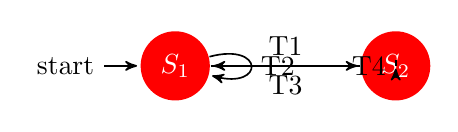
\begin{tikzpicture}[->,>=stealth',shorten >=1pt,auto,node distance=2.8cm,semithick]
				
           	    \tikzstyle{every state}=[fill=red,draw=none,text=white]
            	\node[initial,state] (A) {$S_1$};
            	\node[state] 		 (B) [right of =A] {$S_2$};
            	
            	\path (A) edge   node {T1} (B)
            			edge [loop right]  node{T2} (A)
            	
            		  (B) edge     node {T3} (A)
            				edge  node {T4} (B);
            \end{tikzpicture}  
            \caption{\label{fsaf} todo make this in dia and fix it}                         
            \end{figure}
            
            \subsubsection{Spliting into sub-sequences}
            Another job of the pre-parser is to analyse the sequence of tokens, now with most of the comments removed, and split the sequence in to sub-sequences recursively exactly three times. This is to allow for easy parsing which will be detailed later
            
            In order to describe these splits I must reiterate the structure of the tablature files. Each file may have multiple "blocks" that may refer to multiple "patterns" which can be be split into individual "lines" which each line pertaining to one drum component, as outlined in figure \ref{fig:tabStruct}.
           
            
            \begin{figure}[h]
			\centerline{\includegraphics[scale=0.5]{figures/PLACEHOLDER.eps}}
			\caption{\label{fig:tabStruct} Here depicts the structure of a }
\end{figure}

			The first split, therefore, deals with splitting the file into these "blocks". This is done quite simply by looking for cases where \emph{NewLine} tokens occur repeatedly after populating a block, i.e. if the number of \emph{Newline} tokens excedes one (the one used to seperate lines within a block) before another token is encountered then we have reached the end of the block we are currently building.
			
			The next split is splitting each block into lines, this is done by splitting each block sequence on \emph{NewLine} tokens. This is counter-intuitive to the concept of the how the tablature is grouped but due to a need to verify the patterns this must be done first. This is done by veryfying that each line is of the same length as the rest. If not then the whole block is discarded as we assume it is corrupt.
			
			The final split is that of the individual patterns. Each line is now split on the \emph{TrackDivider} tokens. The first segment of each line is expected to map to the drum component, with the successive segments representing the beats and rests of the pattern. todo possible diagram?
			
			
		\subsection{Parsing}
			Due to all this pre-precessing the job of converting the 4 level sequences representing each drum tablature file, which was built in the previous step, to a datastructure that we can match against is very simple.
			
			Before I outline the method for parsing the pre-processed sequences I must first outline the structure the data will be stored in.
			
			\subsubsection{Sequence Specifications}
				I introduce the concept of sequence specifications. These specifications represent a simplified view of a drum rhythm, depicted in figure \ref{fig:seqSpec}.
				
            \begin{figure}[h]
			\centerline{\includegraphics[scale=0.5]{figures/PLACEHOLDER.eps}}
			\caption{\label{fig:seqSpec} Here depicts the structure of a }
\end{figure}

				Each specification has a constant 8 rows, each mapping to one of the 8 drum components discussed in \ref{Midi}. The number of columns is determined by the resolution of the system, for this project I have chosen it to be 16 meaning that we are only looking for patterns that have 16 time divisions, reasons and consequences for doing so will be discussed in the Evaluation todo section?
				
				In each cell of this chart there are two possible values:
					\begin{itemize}
						\item{\textbf{1} - Representing a Beat impulse}
						\item{\textbf{0} - Representing a Rest event (lack of a beat impulse)}
					\end{itemize}
					
				This simplified notation therefore only depicts the \emph{reletive} timing information of the system and a lot of information is removed including power, special notes, and multiple beats within one time division are abstracted away, which again will be discussed in detail in the Evaluation chapter.
				
				\subsubsection{Parsing to sequence specifications}
				
				The job of the parser is now to create these sequence specifications based on the grouped data that was passed to it by the pre-parser. The method for doing so is outlined in algorithm \ref{algo:Parse}.
				
				\begin{algorithm}
				\caption{Parsing the pre-processed tokens}
				\label{algo:Parse}
				\begin{algorithmic}[1]
					\Procedure{BuildSuffixTree}{GroupedTokens gt}
						\State{sequences = empty indexed list of Sequence Specifications}
						\For{each Track t in gt}
							\For{each Line l in t}
								\State{currentInstrument = l.get(0).get(0)}
								\For{i from 1 to l.size()}
									\Comment{For every sequence segment in the line}
									\State{sequenceSegment = l.get(i)}
									\State{Add sequenceSegment to the corresponding Sequence Specification in sequences (or create a new one) by looking at the position in the line (i) and looking at currentInstrument to know which row to of the Specification to add it to}
								\EndFor
							\EndFor
						\EndFor
						
					

					\EndProcedure
				\end{algorithmic}
				\end{algorithm}
				
				One step that is masked in this algorithm in the actual implementation is that only sequenceSegments that fit the resolution of the system are added. This is to simplify the pattern matching process later. Due to the way the nature of drum tablature (see todo relevent section) this step will not result in incorrect parses of patterns, as if one sequence segment is of an incompatable resolution then all other segments will be of the same incompatable resolution. Leading to whole sequences being ignored, which means we get a smaller database but still one with integrity.
		\subsection{Information lost}
					As discussed in (todo ref relevent section) ASCII Drum Tablature has a lot of superfolous information that cannot be retrieved without significant natural language processing. Furthermore due to the lack of a standardised practice in terms of formatting, and symbol use, a large subset of the drum tablature cannot be harvested without a significantly more complicated parser. As this was not the focus of the project I decided to create a solution that would serve to create a decent database rather than one that solves the general case.
		todo move to evaluation?
	\section{Inference Module}

	In order to extract and infer the pattern the user intended to play the Inference module has the following pipeline.

	\begin{itemize}
		\item{Split the recording into eight note channels representing each drum component}
		\item{Calculate the time deltas between each drum beat on each channel}
		\item{Form a suffix tree, for each note channel, using these time deltas (rounded to some increment) as the alphabet}
		\item{Find the repeated sequence that fits best}
		\item{Extract the inferred pattern}
		\item{Rank the patterns in the database in order of best fit}
		\item{Return both the inferred pattern and this ordered list of matches to user}
	\end{itemize}
	
	The first two steps are justified and explained in \ref{Midi}. The successive steps are explained in detail here.
		\subsection{\label{subsec:SuffixTree}Suffix Tree's}
		A suffix tree, as discussed in \ref{subsec:PrepSuffix}, is a data structure that will help in discovering repeated structure in each note channel. Gusfield's\cite{Gusfield1999} description of the data structure formed the basis for the implementation, along with the basis for the repeated structure extraction algorithm.
		
			\subsubsection{Definition of Suffix Tree's}
			Given a string $S$ of length $n$ a suffix tree is said to be defined as:
			\begin{itemize}
				\item{A tree with exactly $n$ leaves labelled $0$ to $n-1$}
				\item{Internal nodes\footnote{Internal nodes are non-leaf, non-root nodes} have at least two children}
				\item{Each edge is labelled with a non empty sub-string of $S$}
				\item{The starting character of the label of each edge coming out of a node is unique}
				\item{Concatenating each path from root to leaf, which is labelled with $i$, gives the sub-string from $i$ to $n$, i.e. the suffix starting at index $i$}
\end{itemize}
			
			To ensure that no suffix is a prefix of another, a terminal symbol that is not expected to be seen in the string is used to pad S. In the literature this is usually denoted as '\$' though in practice it can be anything that is known to not occur. For this purpose I reserved the time delta '-1' for use as the terminal symbol.

			Because of this, all tree's in my implementation will have $n+1$ leaf nodes. Furthermore, as all \emph{internal nodes} have at least two children there can be at most $n$ such nodes. So with 1 root node there can be at most $(n+1)+n+1 = 2n+2$ (todo double check this) nodes in total.
			
			However, this definition requires $O(n\textsuperscript{2})$ space due to the labelling of edges with the sub-strings (point 3). In order to remedy this I introduce the concept of \emph{Index pointers}. These are tuples of the form \emph{(start, end)} representing the start and end point of the substring labelling the edge. This compacts the space requirement to $\Theta(1)$ for each edge.
			
			This leads to the conclusion that it is possible to represent the Suffix tree in $\Theta(n)$ space, and therefore, for large values of $n$, the overhead for representing the the sequence as a tree is negligible.
			
			\subsection{\label{subsubsec:Ukonnens}Suffix Tree Construction: Ukonnens Algorithm}
			Representing the tree in linear space is not enough for the performance of the system. It is also important for the system to be able to construct the trees in linear time. Furthermore, it will be ideal if the system can update the tree on-line\footnote{Meaning at most one step per character} to agree with the aim of developing a system that can be trivially extended to work in real-time. Ukkonnen\cite{Ukkonen1995} developed an algorithm that does all these things, which will be the basis for my implementation of suffix tree construction.
			
			\subsubsection{Implicit suffix tree}
				The first concept that I will introduce is that of an \emph{implicit suffix tree}. If we have a suffix tree T for the sequence S\$, which is the sequence S terminated by ther terminal character \$, the \emph{implicit} suffix tree for sequence S is formed by removing every copy of \$ from the edge labels of the tree, then removing any edge that has no label and removing any node that does not have atleast two children. This is depicted in figure \ref{fig:implicitSuffixTree}
				
				\begin{figure}[h]
			\centerline{\includegraphics[scale=0.5]{figures/PLACEHOLDER.eps}}
			\caption{\label{fig:implicitSuffixTree} Here is the Suffix tree for S\$ and implicit suffix tree for S}
\end{figure}

				Further to this, a implicit suffix tree for any sub-sequence S[0..i] of S can be formed by taking the suffix tree for S[0..i]\$ and deleting the same required labels, edges, and nodes. This implicit suffix tree is notated as $T_i$.
				
				The name for this structure stems from the fact that, while all the information for a sequence is encoded in an implicit suffix tree, it may be just that - \emph{implicit}. This implicity happens when one of the suffix's is prefixed by another, leading to only one path where there would otherwise be two. This is important when we define the 'extendTree(int i)' function later, but for now just keep in mind that each step, i, of the algorithm constructs the implicit suffix tree $T_i$.
				
				\subsubsection{Overview of algorithm}
				The overview of the algorithm is very simple, as seen in algorithm \ref{algo:Ukonnen}, though there are many concepts that are hidden by this higher view that looks like, at first glance, it would run in $O(n^2)$ time. For much of this discussion we borrow Gusfields\cite{Gusfeild1999} definitions of the concepts.
				
				\begin{algorithm}
				\caption{High-level view of Ukkonen's algorithm provided by Gusfield\cite{Gusfield1975}}
				\label{algo:Ukonnen}
				\begin{algorithmic}[1]
					\Procedure{BuildSuffixTree}{Sequence S}
						\State Construct $T_i$
						\State n = length of S
						\For{i from 1 to n-1}
							\State{begin {phase i+1}}
							\For{j from 1 to i+1}
								\State{Begin {extension j}}
								\State{Find the end of the path from the root labeled S[j..i] in the current tree. If needed, extend the path by adding character S(i+1), thus assuring that string S[j..i+1] is in the tree (possibly implicitly).}
								

						\EndFor


					\EndProcedure
				\end{algorithmic}
				\end{algorithm}
				
				
				
				\subsubsection{Suffix extension rules}
				In order to define the important details of the extension stages of algorithm \ref{algo:Ukonnen} 
			\subsection{Finding repeated Structures}
			Once the suffix tree has been built it is a simple problem to find the repeated structures from it as each internal path\footnote{Internal paths are paths starting at the root and ending at an internal node} corresponds to a repeated point. For this I implemented a simple DFS\footnote{Depth-First Search} algorithm
			todo finish here

			
		\subsection{Bar inferrence}
		Now we have the repeated structures for each note channel. I explored a few options 
			\subsubsection{Quantisation}
			Quantisation is the process of 
	\section{Distance metrics}
	todo write short intro discussing what we have so far (a database of 8x16 strings and a candidate 8x16 string)
	
	In order to apply these algorithms to this domain it is appropiate to consider each row of the strings as sperate to the others. Therefore the overall edit distance for the drum patterns is the sum of the individual edit distances
	
	\subsection{Hamming Distance}
		The Hamming distance\cite{Hamming1950} between two strings, of equal length, measures the minimum number of substitutions in order to change one string into the other. The algorithm, shown in Algorithm \ref{algo:Hamming}, computes the Hamming distance in $O(n)$ time where n is the length of one of the sequences. It is important to note here that the traditional Hamming distance is not defined for strings of unequal length, though given the domain we will never deal with strings of unequal length so there is no need to extend the algorithm.
		\begin{algorithm}
			\caption{Algorithm for computing the Hamming distance between two strings}
			\label{algo:Hamming}
			\begin{algorithmic}[1]
			\Procedure{hammingDistance}{Sequence A, Sequence B}
				\State distance = 0
				\For{i from 0 to lengthOf(A)}
					\If{A.get(i) does not equal B.get(i)}
						\State{distance = distance+1}
					\EndIf
				\EndFor
				\State \Return distance
			\EndProcedure
			\end{algorithmic}
		\end{algorithm}
		
		
 		\subsection{Edit distance}
		The edit distance between two strings is informally defined as the number of edits to get from one of the strings to another. The so called edits in this case are defined by Levenshtein\cite{Levenshtein1966} as insertions, deletions, and substitutions of individual characters. 
		
		A dynamic programming algorithm for computing the edit distance of two strings one dimensional of lengths $m$ and $n$ was devised by Wagner-Fischer in 1974\cite{WagnerFischer1974} which computes the edit distance in $O(nm)$ time and space as seen in Algorithm \ref{algo:WagnerFischer}. 
		
		The advantage the Edit distance has over the Hamming distance is that it does not over penalise for (todo finish comparison).
		
		(todo possibly more detailed explanation of how WagnerFischer works)
		
		\begin{algorithm}
				\caption{Wagner-Fischer algorithm for computing the Edit distance of two strings}
				\label{algo:WagnerFischer}
				\begin{algorithmic}[1]
					\Procedure{editDistance}{Sequence A,Sequence B}
						\State m = lengthOf(A)
						\State n = lengthOf(B)
						\State distances = new 2D array of dimensions (m,n)		
						\State \\initiate the edges of the array
						\For{i from 0 to m}
							
							\State{distances[i][0] = i}
						\EndFor
						\For{i from 0 to n}
							\State{distances[0][i] = i}
						\EndFor
						
						\State \\Now populate the remainder of the array
						\For{j from 1 to n}
							\For{i from 1 to m}
								\If{A.get(i) equals B.get(j)} 
									\Comment{No need edits needed}
									\State{distances[i][j] = distances[i-1][j-1]}
								\Else
									\Comment{Take minimum of operations}
									\State{distances[i][j] = MIN(distances,i,j)}
									
								\EndIf
							\EndFor
						\EndFor
						
						\State \Return distances[m-1][n-1]


					\EndProcedure
					\Procedure{min}{int[][] array,int i, int j}
						\State deletion = array[i-1][j]
						\State insertion = array[i][j-1]
						\State substitution = array[i-1][j-1]
						\State \Return smallestOf(deletion,insertion,substitution)+1
					\EndProcedure
				\end{algorithmic}
				\end{algorithm}
		
		
		\subsection{Cyclic extensions}
		(todo some justification for why a cyclic extension is needed)
		
		In order to extend the distance metrics to find the best match regardless of whether the bar is inferred offset from itself
	\section{Summary}
	

\cleardoublepage
\chapter{Evaluation}
	\section{Comparison with original aims}
	
	\section{Dataset collection}

	\section{Testing}
		repeated sequence vs single recording
		repeated sequence vs repeated with experimentation
	
	\section{Performance Analysis}
	talk about the performance of the harvester
	talk about using sibling lists in suffix trees and alphabet size
	
	\section{Summary}
	
\cleardoublepage
\chapter{Conclusion}
	\section{Lessons learnt}
	\section{Future work}

\cleardoublepage

%%%%%%%%%%%%%%%%%%%%%%%%%%%%%%%%%%%%%%%%%%%%%%%%%%%%%%%%%%%%%%%%%%%%%
% the bibliography

\addcontentsline{toc}{chapter}{Bibliography}
\bibliography{refs}
\begin{thebibliography}{99}
	\bibitem{Shazam}
	Wang, Avery.
	\emph{The Shazam music recognition service},
	Communications of the ACM,
	2006.
	\bibitem{Goto2001}
	Goto, Masataka.
	\emph{An audio-based real-time beat tracking system for music with or without drum-sounds},
	Journal of New Music Research,
	2001.
	\bibitem{Ellis2007}
	Ellis, Daniel PW.
	\emph{Beat tracking by dynamic programming},
	Journal of New Music Reasearch,
	2007.
	\bibitem{EllisPoliner2007}
	Ellis, Daniel PW; Poliner, Graham E.
	\emph{Identifying cover songs' with chroma features and dynamic programming beat tracking}
	Acoustics, Speech and Signal Processing,
	2007.
	\bibitem{DaviesPlumbley2007}
	Davies, Matthew EP; Plumbley, Mark D.
	\emph{Context-dependent beat tracking of musical audio}
	Audio, Speech, and Language Processing,
	2007.
	\bibitem{Mathews1963}
	Mathews, Max.
	\emph{The Digital Computer as a Musical Instrument},
	Science,
	1963.
	\bibitem{Midi1995}
	Rothstein, Joseph.
	\emph{Midi: A comprehensive introduction}
	AR Editions,
	1995.
	\bibitem{BainbridgeBell2001}
	Bainbridge, David; Bell, Tim.
	\emph{The challenge of optical music recognition}
	Computers and Humanities,
	2001
	\bibitem{ComputerMusic}
	Dodge, Charles; Thomas A. Jerse.
	\emph{Computer music: synthesis, composition and performance},
	Macmillan Library Reference, 
	1997.
	\bibitem{Scelta}
	Scelta, Gabriella F.
	\emph{The History and Evolution of the Musical Symbol}.
	\bibitem{Weinberg1994}
	Weinberg, Norman.
	\emph{Guidelines for Drumset Notation},
	Percussive Notes,
	1994.
	\bibitem{Johansen2009}
	Johansen, Linn S.
	\emph{Optical music recognition},
	2009.	
	\bibitem{Knowles2013}
	Knowles, Evan.
	\emph{Parsing Guitar Tab},
	http://knowles.co.za/parsing-guitar-tab/,
	2013.
	\bibitem{CSIRAC}
	Doornbusch, Paul.
	\emph{Computer sound synthesis in 1951: the music of CSIRAC},
	Computer Music Journal,
	2004.
	\bibitem{Weiner1973}
	Weiner, Peter.
	\emph{Linear Pattern Matching Algorithms},
	The Rand Corporation,
	1973.
	\bibitem{Gusfield1999}
	Gusfield, Dan.
	\emph{Algorithms on Strings, Trees and Sequences: Computer Science and Computational Biology}
	Cambridge University Press,
	1999.
	\bibitem{Hamming1950}
	Hamming, Richard W.
	\emph{Error detecting and error correcting codes},
	System technical journal,
	1950.
	\bibitem{Levenshtein1966}
	Levenshtein, Vladimir I.
	\emph{Binary coddes capable of correcting deletions, insertions, and reversals},
	Soviet physics doklady,
	1966.
	\bibitem{Ukonen1995}
	Ukkonen, Esko.
	\emph{On-line construction of suffix trees},
	University of Helsinki,
	1995.
	\bibitem{Bird1977}
	Bird, Richard S.
	\emph{Two dimensional pattern matching},
	Information Processing Letters,
	1977.
	\bibitem{MIDI}
	MIDI Manufacturers Association.
	\emph{MIDI Specifications},
	1996. 
	\bibitem{Walker2007}
	Walker, Martin.
	\emph{Solving MIDI Timing Problems},
	Sound on Sound,
	2007.
	\bibitem{Roland}
	Roland.
	\emph{Roland HD-1 V-Drums Lite - Owner's Manual}
	\bibitem{WagnerFischer1974}
	Wagner, Robert A.; Fischer, Michael J.
	\emph{The string-to-string correction problem},
	Journal of the ACM,
	1974.
	


\end{thebibliography}
\cleardoublepage

%%%%%%%%%%%%%%%%%%%%%%%%%%%%%%%%%%%%%%%%%%%%%%%%%%%%%%%%%%%%%%%%%%%%%
% the appendices
\appendix

\end{document}
